%%%%%%%
%\documentclass[preprint,aps,nofootinbib,preprintnumbers,amsmath,amssymb,11pt]{revtex4-2}
\documentclass[prb,twocolumn,11pt]{revtex4-1}
%%

%%
\usepackage{hyperref}
\usepackage{amsthm}
\usepackage{graphicx}
\usepackage{amsfonts}
\usepackage[figuresright]{rotating}
\usepackage{amssymb}
\usepackage{amsmath}
\usepackage{psfrag}
\usepackage{subfigure}
\usepackage{wrapfig}
\usepackage{multirow}
\usepackage{tabularx}
\usepackage{float}
\usepackage{epsfig}
% \graphicspath{ {images/} }
\usepackage{amsmath}
\usepackage{amssymb}
\usepackage{amsfonts}
\usepackage{graphicx}% Include figure files
\usepackage{dcolumn}% Align table columns on decimal point
\usepackage{bm}% bold math
\usepackage{natbib}
\usepackage{xcolor}
%\textwidth=6.0in 
\newcommand{\half}{\frac{1}{2}}
\newcommand{\beq}{\begin{equation}}
\newcommand{\eq}{\end{equation}}
\newcommand{\bea}{\begin{eqnarray}}
\newcommand{\ea}{\end{eqnarray}}
\newcommand{\p}{\partial}
\newcommand{\nn}{\nonumber}
\newcommand{\Rm}{\mathbb{R}}
\linespread{1.1}

\def\avg#1{\langle#1\rangle}
\def\Re {\mbox{Re}}
\def\Im {\mbox{Im}}
\def\tr{\mbox{tr}}
\def\nn{\nonumber}
\def\pp{\parallel}
\def\c{\hspace{2pt}}
\def\cN{{{\cal N}}}

\newcommand{\SR}[1]{{\color{red} [SR: #1]}}

\begin{document}



\def\thesection{\arabic{section}}
\def\thesubsection{\arabic{section}.\arabic{subsection}}
\numberwithin{equation}{section}

\onecolumngrid
\begin{center}
{\Large {\bf Three-point correlation functions of critical system}}
\vspace{10pt}

{\Large
\bigskip
Junchen Rong
}
{\\~
\\CPHT, CNRS, \'Ecole Polytechnique, Institut Polytechnique de Paris, Palaiseau, France}
\end{center}
\section{Introduction}
At the critical point, the two-point function and three-point correlation function of operators look like~\cite{polyakov1969microscopic},
\begin{align}
\langle\sigma(x)\sigma(y)\rangle &= \frac{c_1}{|x-y|^{2\Delta_{\sigma}}}, \quad {\rm with} \quad |x-y|:=\sqrt{\sum_i (x^i-y^i)^2}.\nonumber\\
\langle\sigma(x_1)\sigma(x_2)\epsilon(x_3)\rangle &=\frac{c_2}{|x_1-x_2|^{2\Delta_{\sigma}-\Delta_{\epsilon}}|x_1-x_3|^{\Delta_{\sigma}}|x_2-x_3|^{\Delta_{\sigma}}}.
\end{align}
Here, $c_1$ and $c_2$ are arbitrary constants and $\Delta_{\sigma}$ and $\Delta_{\epsilon}$ are the so-called scaling dimensions, which is related to the critical exponents of the critical system.
The correlation functions above are defined as the connected correlations, such as
\begin{align}
    \langle ABC\rangle= \langle ABC\rangle_0-\langle A\rangle_0\langle BC\rangle_0-\langle B\rangle_0\langle AC\rangle_0-\langle C\rangle_0\langle AB\rangle_0+2 \langle A\rangle_0\langle B\rangle_0 \langle C\rangle_0.
\end{align}

For a quantum spin chain of length $L$ with a periodic boundary condition, the formula get modified to be 
\begin{align}
    \langle\sigma(x_1)\sigma(x_2)\rangle& = c_1\left|\frac{1}{2L\sin(\frac{\pi|x_1-x_2|}{L})}\right|^{2\Delta_{\sigma}}\nonumber\\
\langle\sigma(x_1)\sigma(x_2)\epsilon(x_3)\rangle&=c_2 \frac{1}{\bigg|2L\sin(\frac{\pi|x_1-x_2|}{L})\bigg|^{2\Delta_\sigma-\Delta_\epsilon}\bigg|2L\sin(\frac{\pi|x_2-x_3|}{L})\bigg|^{\Delta_\epsilon}\bigg|2L\sin(\frac{\pi|x_1-x_3|}{L})\bigg|^{\Delta_\epsilon}}
\end{align}
Now the bracket denotes the vacuum expectation values. These are predictions from conformal symmetry; our goal is to verify these formulas. 
\section{Transverse field Ising model and DMRG}
We can check these predictions using the DMRG simulation of the transverse field Ising model. 
The transverse field Ising model has the Hamiltonian
\begin{equation}
    \hat{H}=-J \sum_{i} Z_i Z_{i+1}+h \sum_i X_i.
\end{equation}
We define it on a one-dimensional spin chain, with a periodic boundary condition. When $h>J$, the system is in the disordered phase. When $h<J$, the system is in the spontaneous symmetry-breaking phase. The critical point is at $h=J$, which is described by the two-dimensional Ising CFT.
We use DMRG to calculate the ground state wave function at the critical point, and then measure the correlation function. 
To compare with the lattice result, we need to identify the lattice operators with CFT operators
\begin{align}
    \sigma_i \sim Z_i,\nonumber\\
    \epsilon_i \sim X_i.
\end{align}
We consider a spin chain with length $L=40$. When calculating the three-point function, we set $x_1=1$, $x_2=11$, and vary $x_3$.
The results are summarized in Fig. \ref{correlations}. 
\begin{figure}[htbp]
\centering
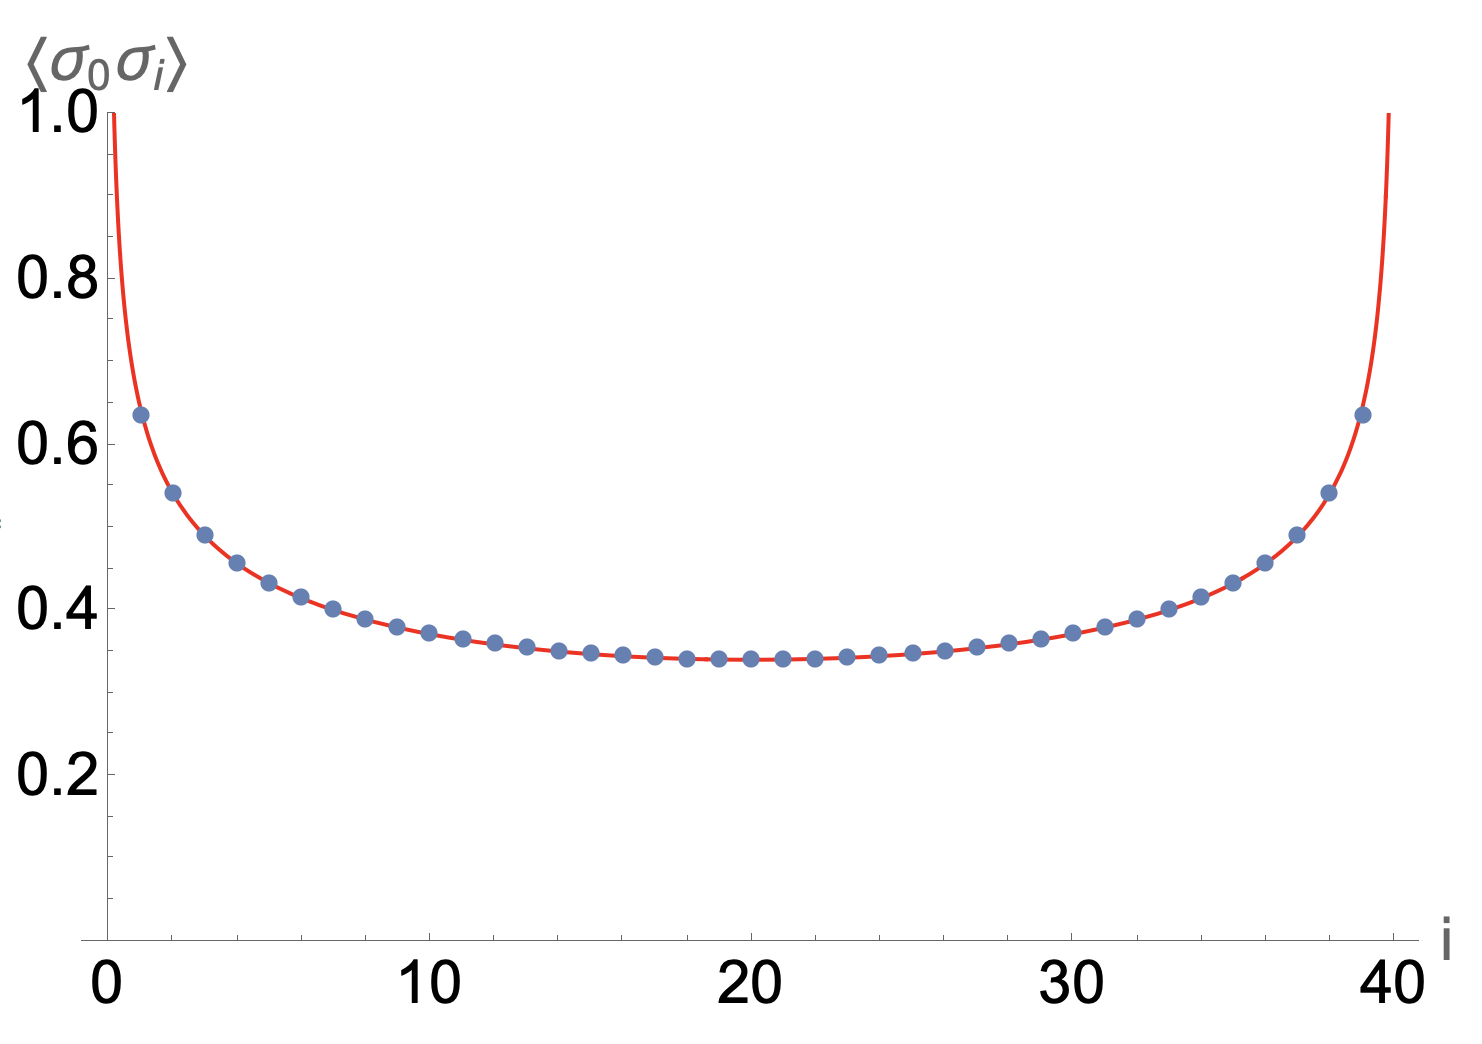
\includegraphics[scale=0.3]{ss2ptIsing.png}
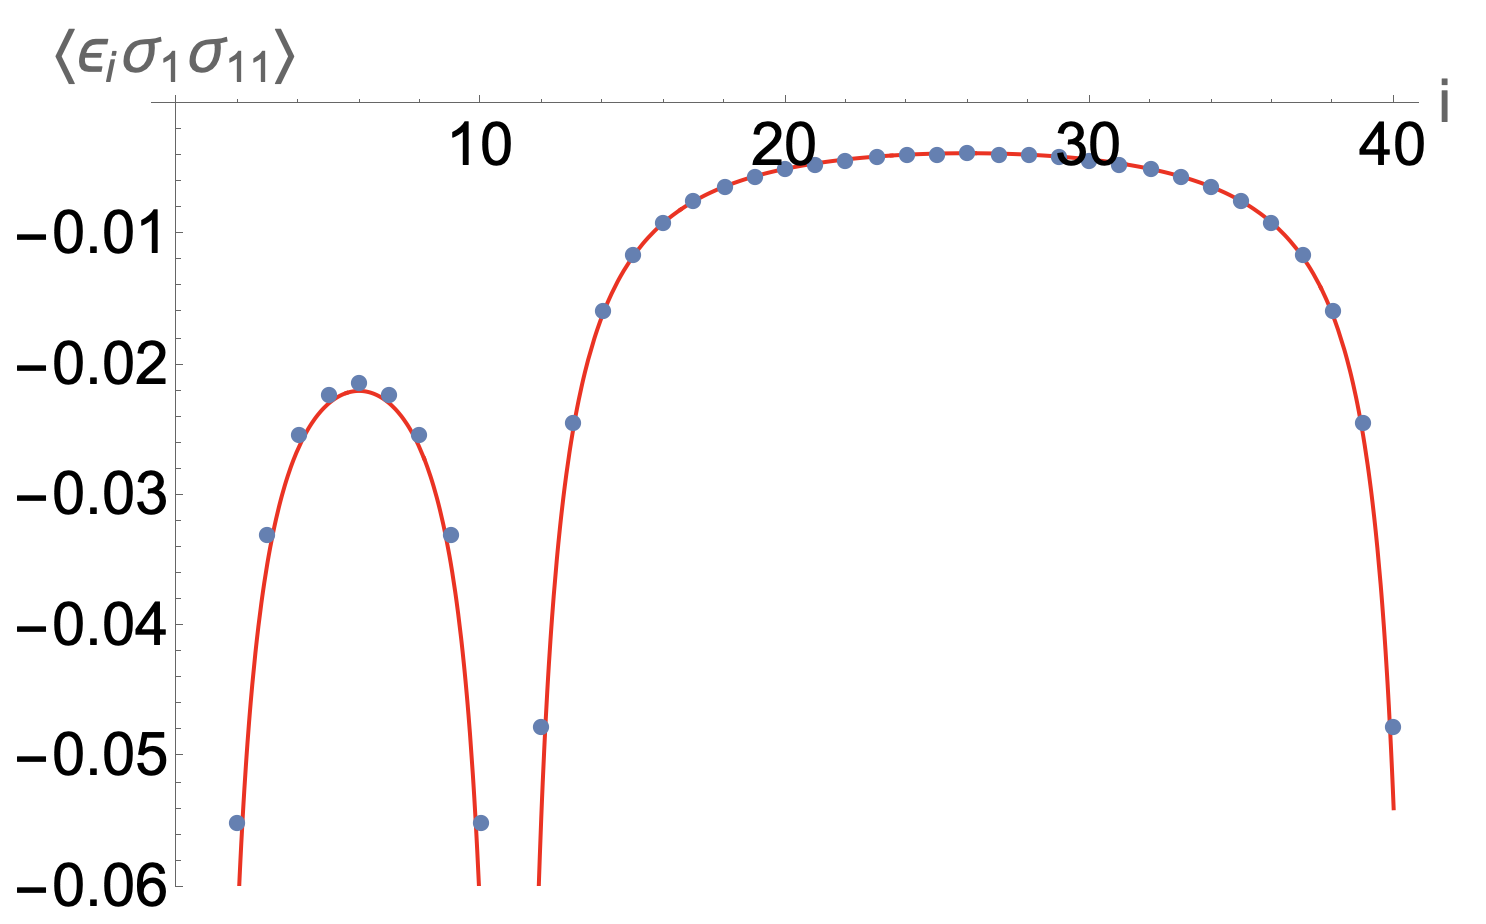
\includegraphics[scale=0.3]{sse3ptIsing.png}
\caption{The two-point $\langle\sigma(x_1)\sigma(x_2)\rangle$ and three-point functions $\langle\epsilon(x_1)\sigma(x_2)\sigma(x_3)\rangle$. The dots are measured at the critical point of the transverse field Ising model, and the red curve is the result predicted by the conformal symmetry. We have used $\Delta_\sigma=\frac{1}{8}$ and $\Delta_{\epsilon}=1$.}
\label{correlations}
\end{figure}
\section{Fendley-Sengupta-Sachdev model}
There exists a model that is closer to the Rydberg atom experiments, called the Fendley-Sengupta-Sachdev model. The Hamiltonian is 
\begin{equation}
    \hat{H}=-J \sum_i (d_i^{\dagger}+d_i)+ U \sum_i n_i + V \sum_i n_{i-1}n_{i+1}.
\end{equation}
There can not be more than one boson occupying the same site, that is 
\begin{equation}
    n_i=0\quad {\rm or} \quad 1.
\end{equation}
In addition to that, the hardcore bosons cannot occupy neighboring sites; this is often called the Rydberg blockade condition, that is 
\begin{equation}
    n_i n_{i+1}=0.
\end{equation}
The phase diagram of this model has been studied using DMRG, see for example~\cite{10.21468/SciPostPhys.6.3.033}.
\begin{figure}[htbp]
\centering
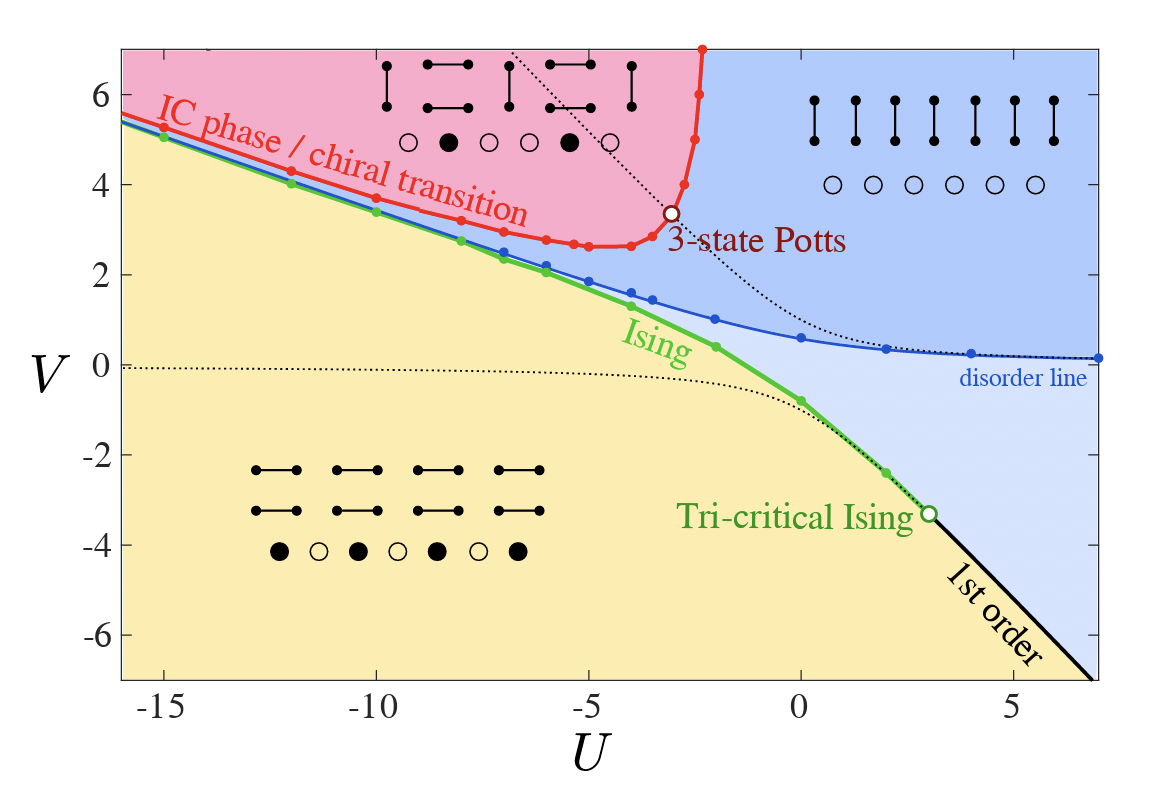
\includegraphics[scale=0.4]{phase_diagram.png}
\caption{The phase diagram of the Fendley-Sengupta-Sachdev model. The plot is reproduced from~\cite{10.21468/SciPostPhys.6.3.033}. }
\label{phasediagram}
\end{figure}
The coupling constants are related to experimental parameters. We identify the ground state of the atom as the state not occupied by the boson $|0\rangle$, and the Rydberg state as the state occupied by the boson $|1\rangle=d^{\dagger}|0\rangle$. 
One can change the coupling $J$ by changing the Rabi frequency of the external laser.
The frequency of the external laser is adjusted so that the detuning away from resonance of the $|0\rangle$ to $|1\rangle$ transition is $U$. 
(See Sachedev's new book ``Quantum Phases of Matter''). We can also replace the last term by a long-range repulsive interaction to represent the van der Waals interaction
when both atoms are in their Rydberg states.

\begin{figure}[h!]
	\centering
	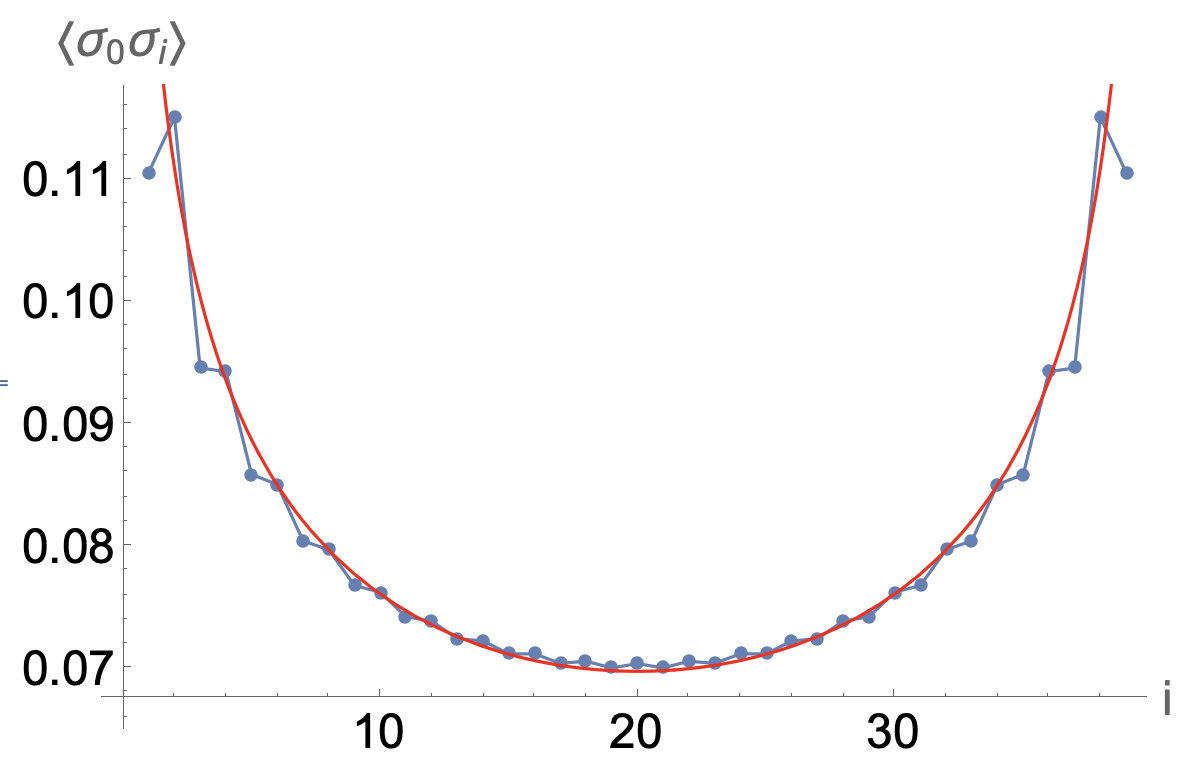
\includegraphics[scale=0.3]{ss2ptHB.png}
	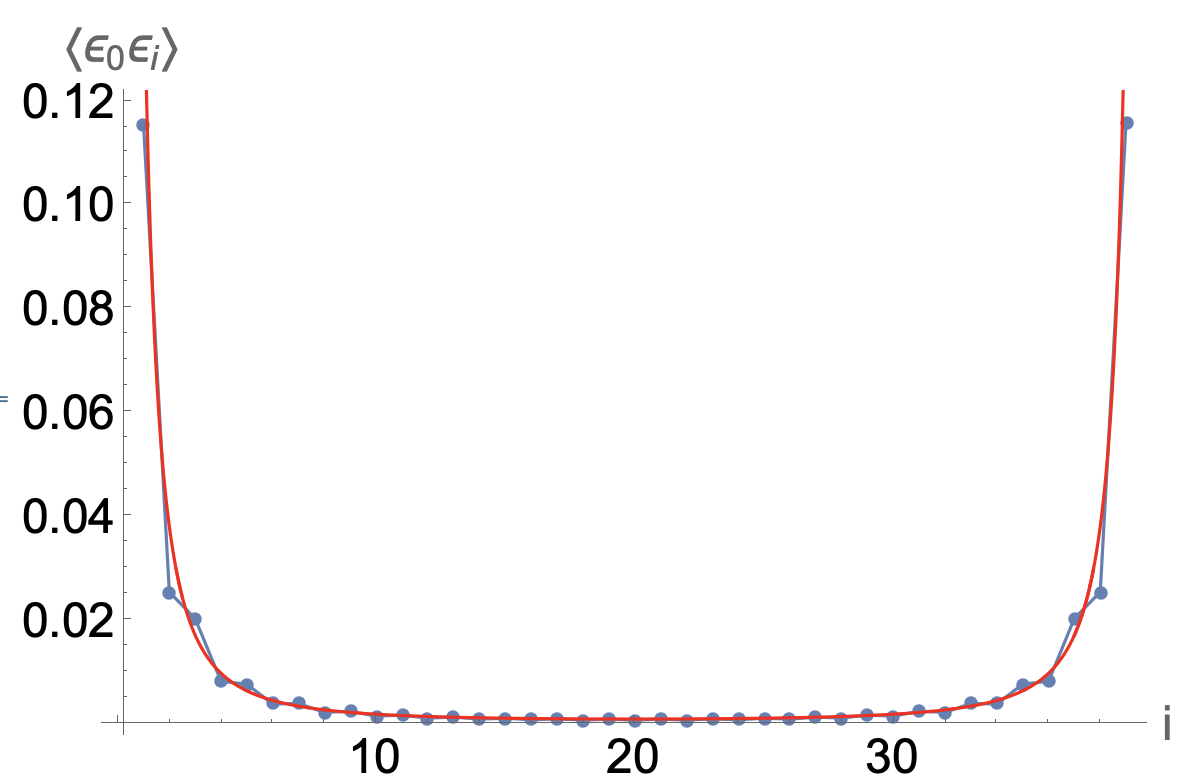
\includegraphics[scale=0.3]{ee2ptHB.png}
	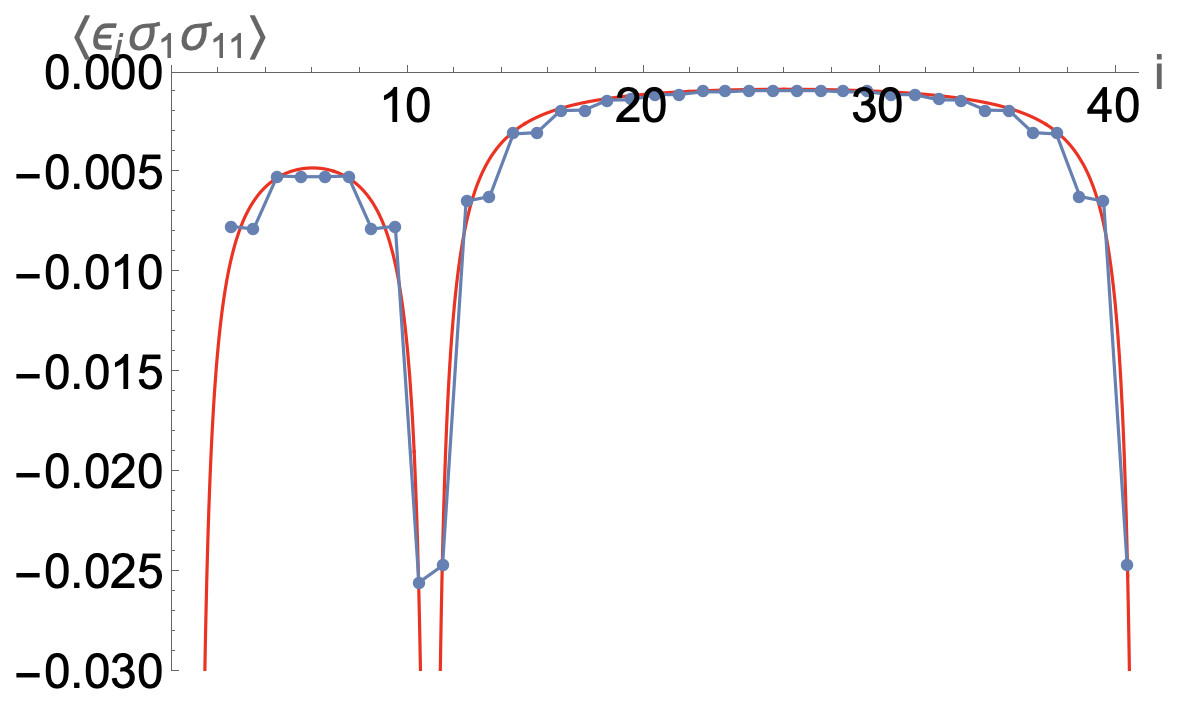
\includegraphics[scale=0.35]{sse3ptHB.png}
	\caption{The two-point and three-point functions of the Fendley-Sengupta-Sachdev model.}
	\label{correlationsHB}
\end{figure}

We can again study this model using DMRG. We can identify 
\begin{align}
    d^{\dagger}+d \quad \rightarrow  \quad X.
\end{align}
Here $X$ is the Pauli Matrix. 
To impose the Rydberg blockade condition, we add a strong repulsive interaction 
\begin{align}
    \hat{H}_{rp}=U_{rp} \sum_i n_i n_{i+1}.
\end{align}
We can also identify the lattice operators with CFT operators according to,
\begin{align}   
    \sigma_i \sim &\quad  (-1)^i n_i \nonumber\\
    \epsilon_{i+1/2} \sim & \quad (1-n_{i})(1-n_{i+1}).
\end{align}
The $\epsilon$ operator is defined on the bonds. 
We study a lattice with $L=40$ sites. We set the coupling constants to be 
\begin{align}
    J=1,\quad U=0.128, \quad V=-1, \quad {\rm and}\quad U_{rp}=20.
\end{align}
The two-point $\langle\sigma_0 \sigma_1\rangle$ and three-point functions  $\langle \epsilon_i \sigma_1 \sigma_{11}\rangle$ can be found in Fig.~\ref{correlationsHB}.


\section{A more realistic model}
Finally, we can consider a more realistic model with van der Waals $1/r^6$ interaction between the excited atoms
\begin{equation}
    \hat{H}=-J \sum_i (d_i^{\dagger}+d_i)+ U \sum_i n_i + V\sum_{ij}\frac{1}{(d_{ij})^6}  n_{i}n_{j}.
\end{equation}
Here $d_{ij}$ is the distance between the $i$-th and $j$-th sites. Since the sites are arranged to form a circle, we take
\begin{align}
    d_{ij}=\frac{\sin(\frac{|i-j|}{L}\pi)}{\sin(\frac{1}{L}\pi)}.
\end{align}
We have normalized the distance so that the distance between neighbouring sites is 1.
We do not need to impose the Rydberg blockade condition in this case.
We find a critical point at
\begin{align}
    J=1,\quad U=-2.15,\quad  V=8.
\end{align}

\SR{I think you promised Antoine the phase diagram}

\SR{below needs to be modified because interchanging spins is not a symmetry of the Hamiltonian}

We can also modify the map between the lattice operators and CFT operators,
\begin{align}
    \sigma_{i+1/2}\sim &~(n_i-n_{i+1}),\nonumber\\
    \epsilon_{i+1/2} \sim &~n_i+n_{i+1}- (1-n_{i})(1-n_{i+1}).
\end{align}
Due to the symmetry-breaking pattern, we treat two neighbouring sites as a single unit cell. The above operators are defined when $i$ is an even integer.
The results are summarized in Fig.~\ref{correlationsHBlong}, for two point and three point functions.
\begin{figure}[htbp]
\centering
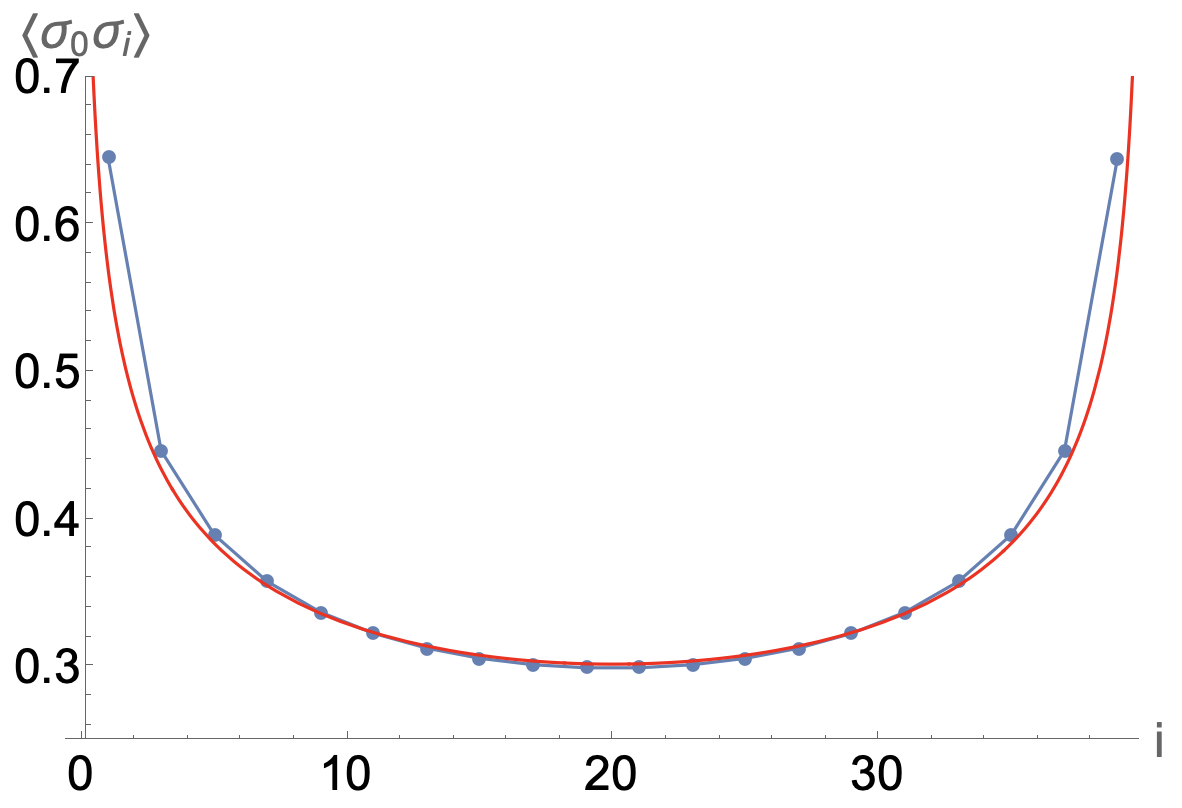
\includegraphics[scale=0.35]{ss_long_range.png}
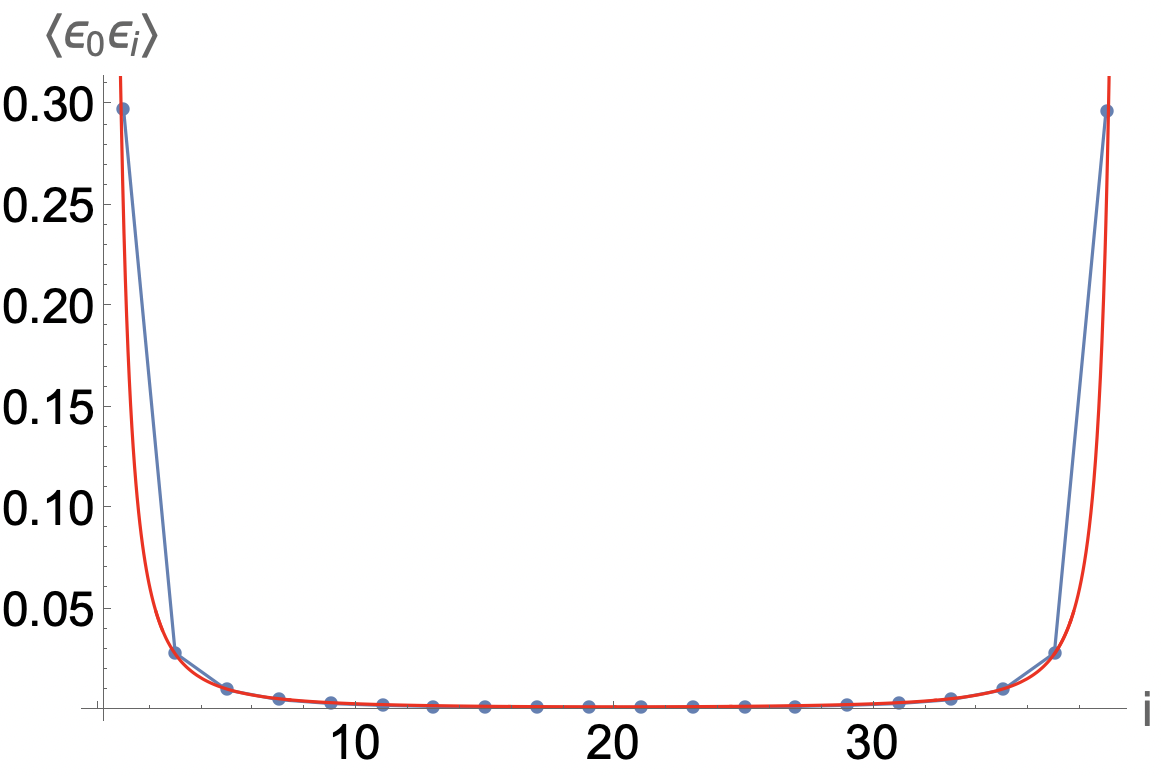
\includegraphics[scale=0.35]{ee_long_range.png}
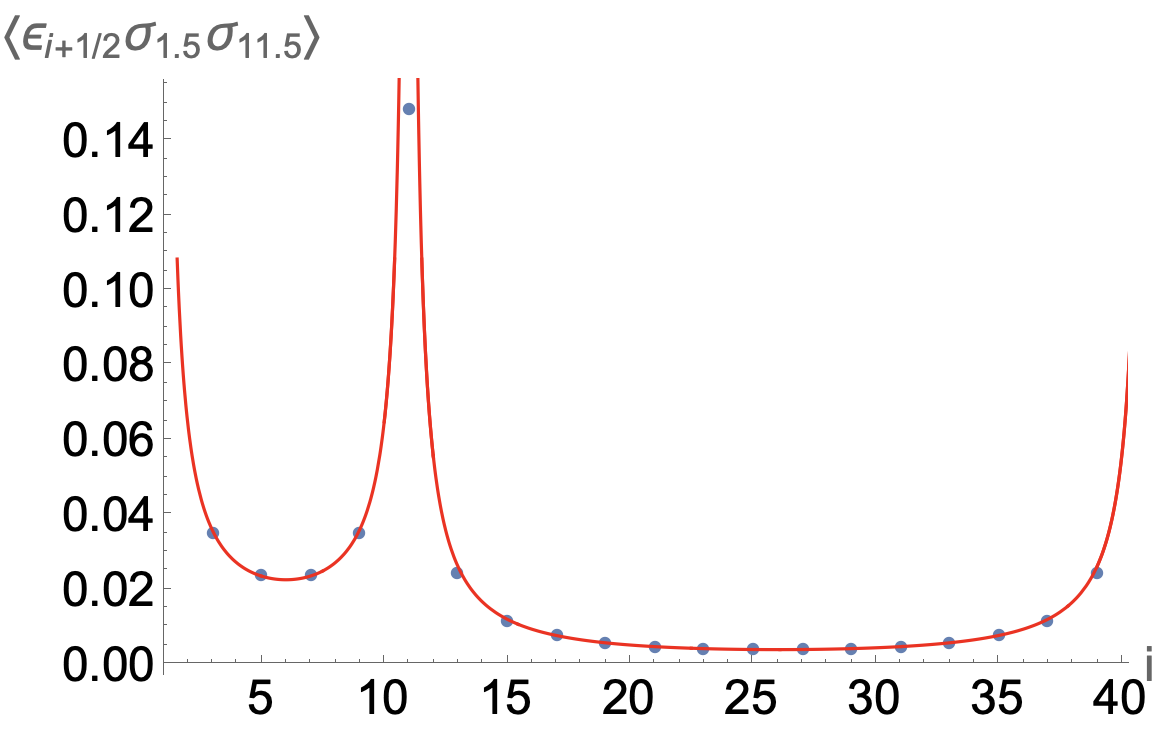
\includegraphics[scale=0.35]{ess_long_range.png}
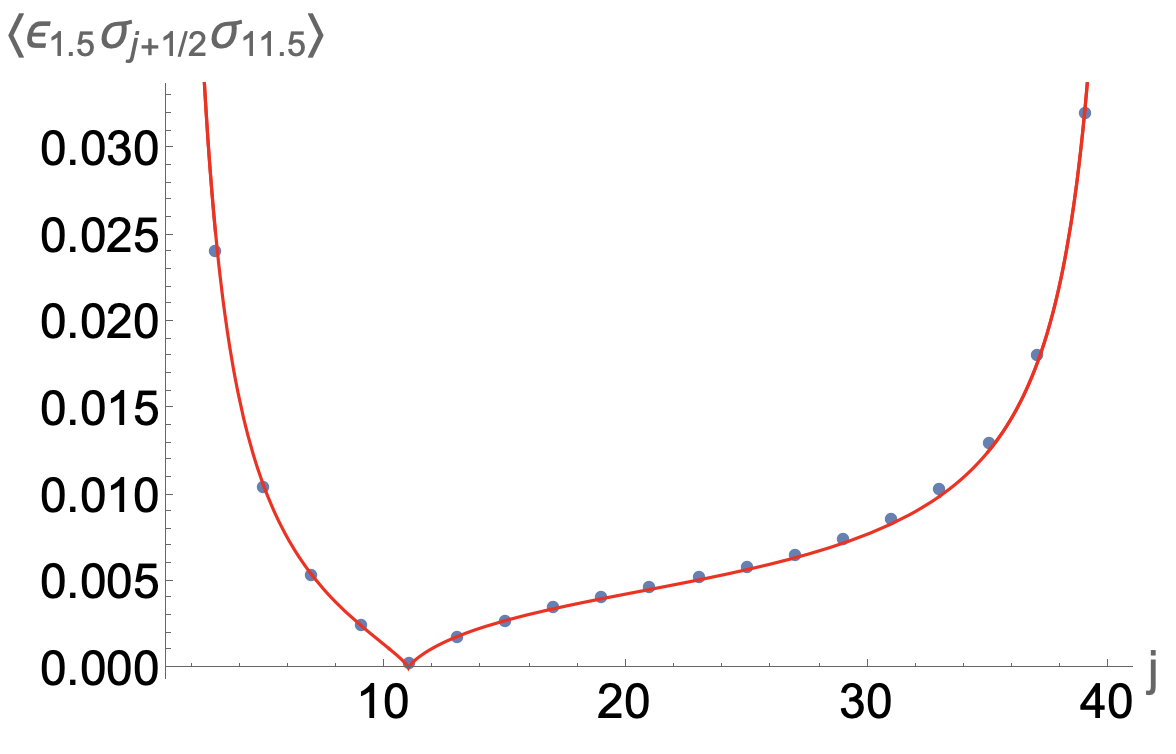
\includegraphics[scale=0.35]{ess_long_range2.png}
\caption{The two-point and three-point functions of the Fendley-Sengupta-Sachdev model with long-range interaction.}
\label{correlationsHBlong}
\end{figure}

%\begin{multicols}{2}
%\twocolumngrid
%\bibliographystyle{JHEP}
\bibliography{reference.bib}
%\end{multicols}
\end{document}



